\section{Dijkstra Algorithm}

\begin{frame}{Dijkstra Algorithm}{Shortest Path without Computer}
  \begin{itemize}
    \item
      Wanted: Shortest path from M to all other points
    \item
      Place pearls on crossings and clamp strings between them
  \end{itemize}
  \begin{figure}
    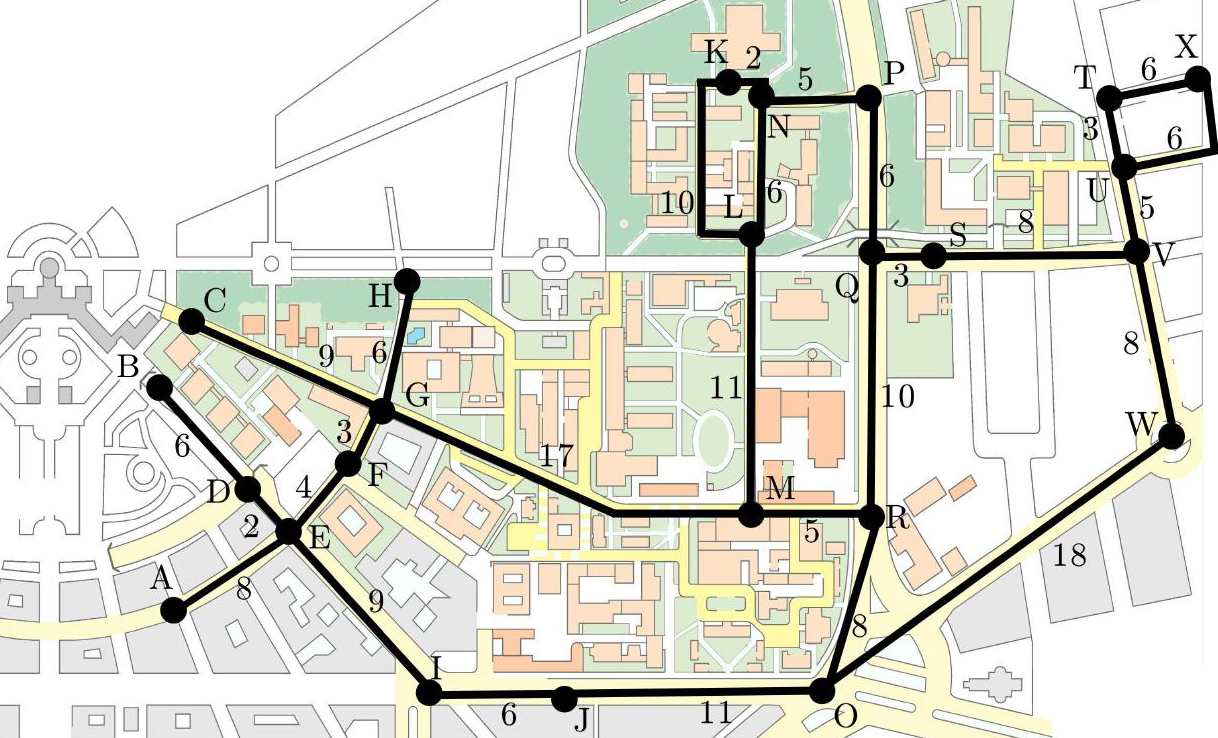
\includegraphics[width=0.75\linewidth]{Images/Dijkstra/DijkstraMap}
    \caption{Map $\copyright\,$ Mehlhorn / Sanders}
  \end{figure}
\end{frame}

%-------------------------------------------------------------------------------

\begin{frame}{Dijkstra Algorithm}{Shortest Path without Computer}
  \vspace{-1.5em}
  \begin{columns}
    \begin{column}{0.55\linewidth}
      \begin{figure}[!t]
        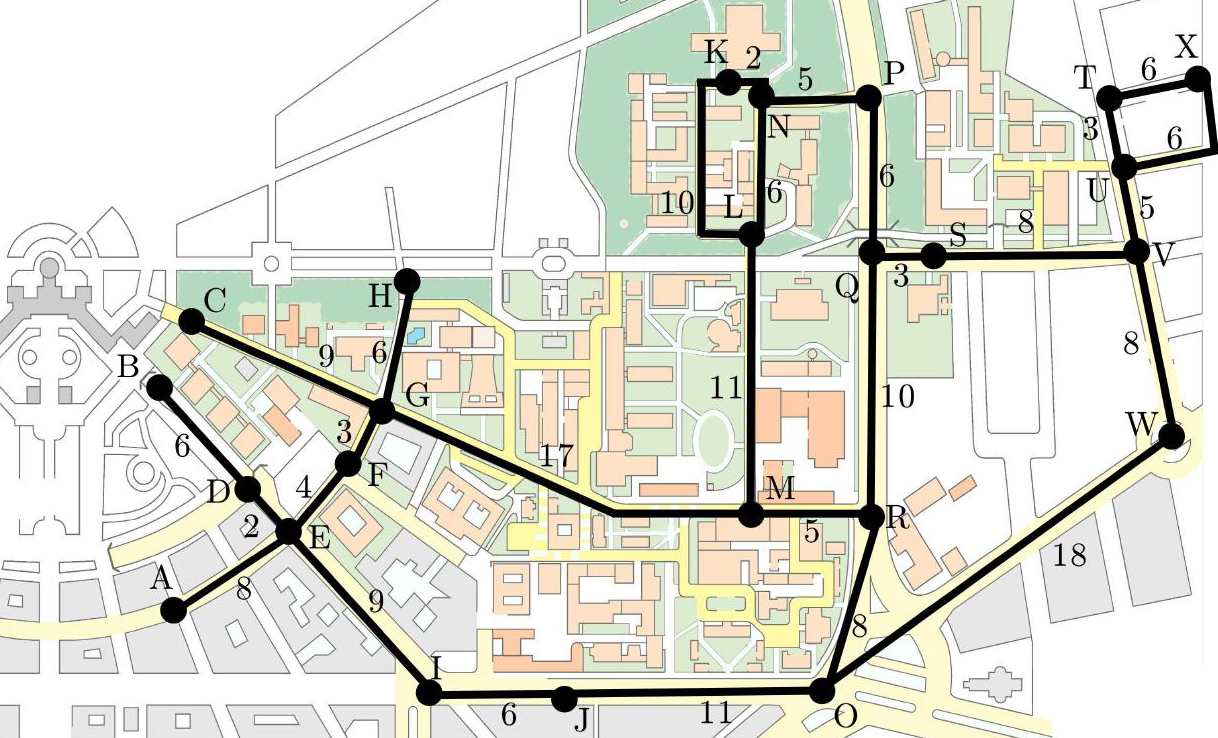
\includegraphics[width=0.8\linewidth]
          {Images/Dijkstra/DijkstraMap}
        \caption{Map $\copyright\,$ Mehlhorn / Sanders}
      \end{figure}
      \vspace{-1.5em}
      \begin{itemize}
        \item
          Take the net and pull it slowly upwards until fully lifted
        \item
          Each node (pearl) now has a specific height
        \item
          The distance to M is exactly the {\color{Mittel-Blau}shortest path}
      \end{itemize}
    \end{column}
    \begin{column}{0.45\linewidth}
      \begin{figure}[!t]
        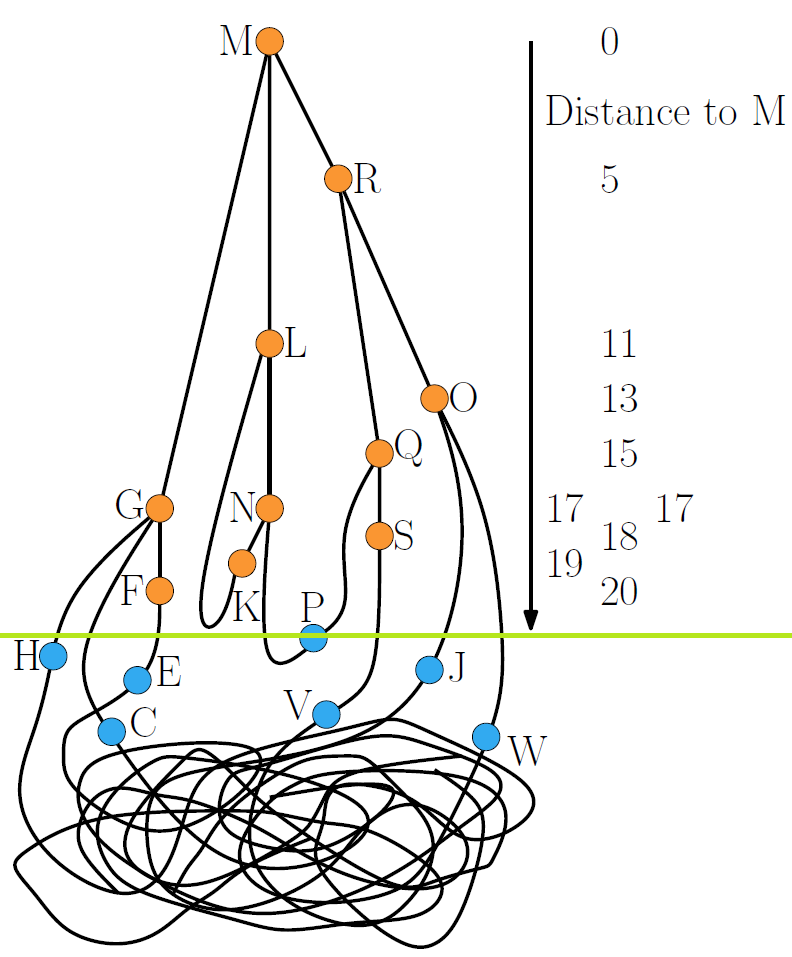
\includegraphics[width=\linewidth]
          {Images/Dijkstra/DijkstraTree_WithOverlay}
        \vspace{-0.5em}
        \caption{Map $\copyright\,$ Mehlhorn / Sanders}
      \end{figure}
    \end{column}
  \end{columns}
\end{frame}


%-------------------------------------------------------------------------------

\begin{frame}{Dijkstra Algorithm}{Shortest Path}
  
\end{frame}